\documentclass[12pt]{article}
\usepackage[margin=1in]{geometry}
\setlength{\parindent}{0pt}
\setlength{\parskip}{5pt}
%\pagenumbering{gobble}% 

\usepackage{amsmath,amsthm,amssymb}
\usepackage{graphicx}
\usepackage{bm}
\usepackage{float}
\usepackage{caption}
\newtheorem{euclidtheorem}{Proposition}[section]
\newtheorem{classtheorem}{Theorem}
\newtheorem{theorem}{Theorem}[section]
\newtheorem{challenge}[theorem]{Challenge}
\newtheorem{question}[theorem]{Question}
\newtheorem{problem}[theorem]{Problem}

\newtheorem{theorempiece}{Theorem}[theorem]
\newtheorem{classtheorempiece}{Theorem}[classtheorem]
\newtheorem{challengepiece}{Challenge}[theorem]
\newtheorem{questionpiece}{Question}[theorem]
\newtheorem{problempiece}{Problem}[theorem]

\renewcommand*{\theeuclidtheorem}{\Roman{section}.\arabic{theorem}}
\renewcommand*{\thetheorem}{\arabic{section}.\arabic{theorem}}
\renewcommand*{\theclasstheorem}{\Alph{theorem}}
\renewcommand*{\thechallenge}{\arabic{section}.\arabic{theorem}}
\renewcommand*{\thequestion}{\arabic{section}.\arabic{theorem}}
\renewcommand*{\theproblem}{\arabic{section}.\arabic{theorem}}
\renewcommand*{\thetheorempiece}{\arabic{section}.\arabic{theorem}.\alph{theorempiece}}
\renewcommand*{\thechallengepiece}{\arabic{section}.\arabic{theorem}.\alph{challengepiece}}
\renewcommand*{\thequestionpiece}{\arabic{section}.\arabic{theorem}.\alph{questionpiece}}
\renewcommand*{\theproblempiece}{\arabic{section}.\arabic{theorem}.\alph{problempiece}}

\usepackage{tikz}
\usepackage{wasysym} 
\usepackage{multicol}
\usepackage{setspace}

\title{Homework 4 of Statistical Machine Learning}
\author{Wang Yikai, 2017310740}
\date{\today}

\begin{document}

\maketitle

{\large \bf 1 Probabilistic Graphical Models}
\bigskip \par
{\bf 1.1 Conditional Queries in a Bayesian Network}
\smallskip\par
1. The probabilistic graph of the model is shown in Figure 1. There are:
\begin{align*}
&P(G_1) = (0.5,0.5),\;
P(G_i|G_1)=
 \left(
 \begin{matrix}
   0.9 & 0.1\\
   0.1 & 0.9
  \end{matrix}
  \right)
,\,(i=2,3)\\
&p(X_i|G_i = 1) = \mathcal{N}(X_i |\mu = 55,\sigma^2 = 10),\, (i = 1,2,3)\\
&p(X_i|G_i = 2) = \mathcal{N}(X_i |\mu = 65,\sigma^2 = 10),\, (i = 1,2,3)
\end{align*}

The {\bf Markov blanket} of $G_3$ contains $G_1$ and $X_3$.
\begin{figure}[ht]
\centering
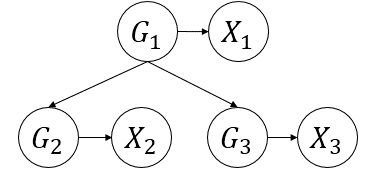
\includegraphics[scale=0.6]{1.png}
\caption{Probabilistic graph}
\end{figure}
\par 
2. Suppose $X_2$ is observed to be $50$. In Python, uses {\bf scipy.stats.norm.pdf([50], 55, np.sqrt(10))}, there is $P(X_2=50|G_2=1)=0.03614$. Similarly, $P(X_2=50|G_2=2)=1.6\times10^{-6}$.
The posterior belief $P(G_1=1|X_2=50)$ is:
\begin{align*}
P(G_1=1|X_2=50)&=\frac{P(G_1=1,X_2=50)}{P(X_2=50)}\\
&\propto P(G_1=1,X_2=50)\\
&=\sum_{i=1}^2 P(G_1=1,G_2=i,X_2=50)\\
&=\sum_{i=1}^2 P(G_1=1)P(G_2=i|G_1=1)P(X_2=50|G_2=i)\\
&=0.5\times0.9\times0.03614 + 0.5\times0.1\times1.6\times10^{-6}=0.0163
\end{align*}
\begin{align*}
P(G_1=2|X_2=50)&\propto P(G_1=2,X_2=50)\\
&=\sum_{i=1}^2 P(G_1=2)P(G_2=i|G_1=2)P(X_2=50|G_2=i)\\
&=0.5\times0.1\times0.03614 + 0.5\times0.9\times1.6\times10^{-6}=0.0018
\end{align*}
As $P(G_1=1|X_2=50)+P(G_1=2|X_2=50)=1$, there are:
$$P(G_1=1|X_2=50)=\frac{0.0163}{0.0163+0.0018}=0.901$$
$$P(G_1=2|X_2=50)=\frac{0.0018}{0.0163+0.0018}=0.099$$

3. Suppose we observe both $X_2 = 50$ and $X_3 = 50$. Then $P(G_1|X_2,X_3)$ is:
\begin{align*}
&P(G_1=1|X_2=50,X_3=50)=\frac{P(G_1=1,X_2=50,X_3=50)}{P(X_2=50,X_3=50)}
\propto P(G_1=1,X_2=50,X_3=50)\\
&=\sum_{i=1}^2\sum_{j=1}^2P(G_1=1)P(G_2=i|G_1=1)P(X_2=50|G_2=i)P(G_3=j|G_1=1)P(X_3=50|G_3=j)\\
&=P(G_1=1)\sum_{i=1}^2[P(G_2=i|G_1=1)P(X_2=50|G_2=i)]\sum_{j=1}^2[P(G_3=j|G_1=1)P(X_3=50|G_3=j)]\\
&=0.5\times(0.9\times0.03614+0.1\times1.6\times10^{-6})^2=5.29\times10^{-4}\\
&P(G_1=2|X_2=50,X_3=50)=0.5\times(0.1\times0.03614+0.9\times1.6\times10^{-6})^2=6.53\times10^{-6}
\end{align*}
As $P(G_1=1|X_2=50,X_3=50)+P(G_1=2|X_2=50,X_3=50)=1$, there are:
\begin{align*}
&P(G_1=1|X_2=50,X_3=50)=\frac{5.29\times10^{-4}}{5.29\times10^{-4}+6.53\times10^{-6}}=0.988\\
&P(G_1=2|X_2=50,X_3=50)=\frac{6.53\times10^{-6}}{5.29\times10^{-4}+6.53\times10^{-6}}=0.012
\end{align*}

\bigskip
{\bf 1.2 Conditional Random Fields}
\smallskip\par
1. The undirected graph and the factor graph of the CRF are shown as Figure 2, 3:
\begin{figure}[ht]
\begin{minipage}[t]{0.5\textwidth}
\centering
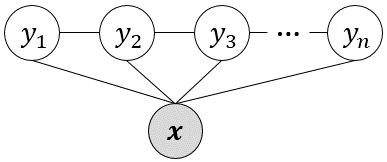
\includegraphics[scale=0.58]{undirected.png}
\caption{Undirected Graph}
\end{minipage}
\begin{minipage}[t]{0.5\textwidth}
\centering
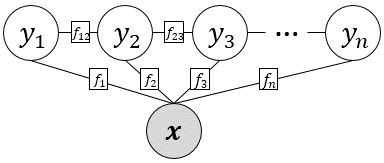
\includegraphics[scale=0.58]{factor_graph.png}
\caption{Factor Graph}
\end{minipage}
\end{figure}
\newpage
2. The cliques of CRF is illustrated as Figure 4.
\begin{figure}[ht]
\centering
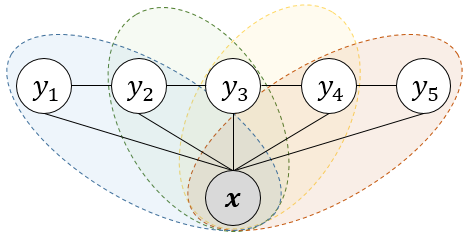
\includegraphics[scale=0.58]{clique.png}
\caption{Cliques of CRF}
\end{figure}
\par
The junction tree of CRF is illustrated as Figure 5.
\begin{figure}[ht]
\centering
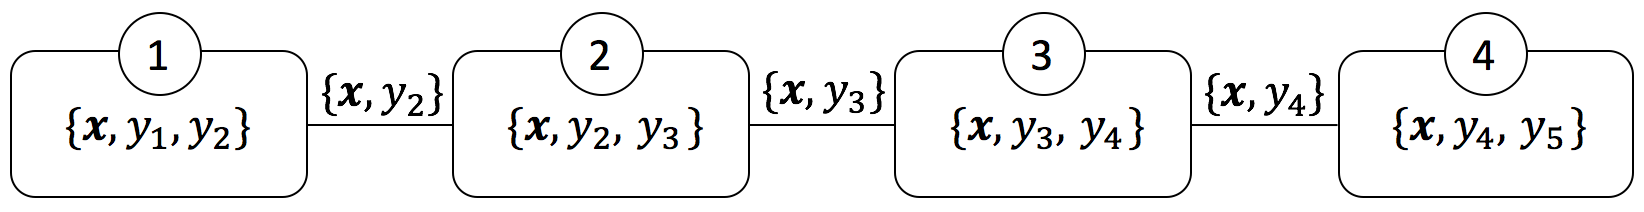
\includegraphics[scale=0.5]{junction_tree.png}
\caption{Junction Tree of CRF}
\end{figure}
\par
Denote each clique in the junction tree as $C_i,i=1,2,3,4$. First, set initial factors at each cluster as products. For example, $\psi_1(\bm{x},y_1,y_2)=\phi(\bm{x},y_1)\phi(y_1,y_2)$.
\par
By running the sum-product algorithm on the junction tree, we can get $p(y_3,\bm x;\bm w)$:
\begin{itemize}
\item In $C_1$, eliminate $y_1$ by sending $\delta_{1\rightarrow2}(\bm{x},y_2)=\sum_{y_1}\psi_1(\bm{x},y_1,y_2)$ to $C_2$;
\item In $C_2$, eliminate $y_2$ by sending $\delta_{2\rightarrow3}(\bm{x},y_3)=\sum_{y_2}\delta_{1\rightarrow2}(\bm{x},y_2)\psi_2(\bm{x},y_2,y_3)$ to $C_3$;
\item In $C_4$, eliminate $y_5$ by sending $\delta_{4\rightarrow3}(\bm{x},y_4)=\sum_{y_5}\psi_4(\bm{x},y_4,y_5)$ to $C_3$;
\item In $C_3$, eliminate $y_4$ to get $p(y_3,\bm x;\bm w)=\sum_{y_4}\delta_{2\rightarrow3}(\bm{x},y_3)\delta_{4\rightarrow3}(\bm{x},y_4)\psi_3(\bm{x},y_3,y_4)$.
\end{itemize}
After getting $p(y_3,\bm x;\bm w)$, there is $p(\bm x;\bm w)=\sum_{y_3}p(y_3,\bm x;\bm w)$. Then by $p(y_3|\bm x;\bm w)=\frac{p(y_3,\bm x;\bm w)}{p(\bm x;\bm w)}$, we can get $p(y_3|\bm x;\bm w)$.

3. Given the following parametric form of CRF:
$$p(\bm{y}|\bm{x};\bm{w})=\frac{1}{Z(\bm{x};\bm{w})}\exp\left\{\bm{w}^T\sum_{i=2}^n\bm{f}(\bm{x},y_i,y_{i-1})\right\}$$
where 
$$Z(\bm{x};\bm{w})=\sum_{\bm{y}'\in\mathcal{L}^n}\exp\left\{\bm{w}^T\sum_{i=2}^n\bm{f}(\bm{x},y_i',y_{i-1}')\right\}$$
To learn the parameters of the CRF, we maximize the conditional log
likelihood of training data $\mathcal{D} =\left\{(\bm{x}^i,\bm{y}^i)\right\}_{i=1}^N$ over parameters $\bm{w}$ using gradient descent:
$$\mathcal{L}(\bm{w})=\sum_{(\bm{x},\bm{y})\in\mathcal{D}}\log p(\bm{y}|\bm{x};\bm{w})=\sum_{(\bm{x},\bm{y})\in\mathcal{D}}\left\{\bm{w}^T\sum_{i=2}^n\bm{f}(\bm{x},y_i,y_{i-1})-\log Z(\bm{x};\bm{w}) \right\}$$
Compute its gradient:
$$\frac{\partial\mathcal{L}}{\partial\bm{w}}=\sum_{(\bm{x},\bm{y})\in\mathcal{D}}\left\{\sum_{i=2}^n\bm{f}(\bm{x},y_i,y_{i-1})-\frac{1}{Z(\bm{x};\bm{w})}\frac{\partial Z(\bm{x};\bm{w})}{\partial\bm{w}}\right\}$$
where $\frac{1}{Z(\bm{x};\bm{w})}\frac{\partial Z(\bm{x};\bm{w})}{\partial\bm{w}}$ is:
\begin{align*}
\frac{1}{Z(\bm{x};\bm{w})}\frac{\partial Z(\bm{x};\bm{w})}{\partial\bm{w}}&=\frac{1}{Z(\bm{x};\bm{w})}\frac{\partial\sum_{\bm{y}'\in\mathcal{L}^n}\exp\left\{\bm{w}^T\sum_{i=2}^n\bm{f}(\bm{x},y_i',y_{i-1}')\right\}}{\partial\bm{w}}\\
&=\frac{1}{Z(\bm{x};\bm{w})}\sum_{\bm{y}'\in\mathcal{L}^n}\exp\left\{\bm{w}^T\sum_{i=2}^n\bm{f}(\bm{x},y_i',y_{i-1}')\right\}\sum_{i=2}^n\bm{f}(\bm{x},y_i',y_{i-1}')\\
&=\sum_{\bm{y}'\in\mathcal{L}^n}\frac{1}{Z(\bm{x};\bm{w})}\exp\left\{\bm{w}^T\sum_{i=2}^n\bm{f}(\bm{x},y_i',y_{i-1}')\right\}\sum_{i=2}^n\bm{f}(\bm{x},y_i',y_{i-1}')\\
&=\sum_{\bm{y}'\in\mathcal{L}^n}p(\bm{y}'|\bm{x};\bm{w})\sum_{i=2}^n\bm{f}(\bm{x},y_i',y_{i-1}')\\
&=\mathbb{E}_{p(\bm{y}'|\bm{x};\bm{w})}\left[\sum_{i=2}^n\bm{f}(\bm{x},y_i',y_{i-1}')\right]
\end{align*}
Therefore $\frac{\partial\mathcal{L}}{\partial\bm{w}}$ is:
\begin{align*}
\frac{\partial\mathcal{L}}{\partial\bm{w}}&=\sum_{(\bm{x},\bm{y})\in\mathcal{D}}\left\{\sum_{i=2}^n\bm{f}(\bm{x},y_i',y_{i-1}')-\mathbb{E}_{p(\bm{y}'|\bm{x};\bm{w})}\left[\sum_{i=2}^n\bm{f}(\bm{x},y_i',y_{i-1}')\right]\right\}\\
&=\sum_{(\bm{x},\bm{y})\in\mathcal{D}}\sum_{i=2}^n\left\{\bm{f}(\bm{x},y_i',y_{i-1}')-\mathbb{E}_{p(\bm{y}'|\bm{x};\bm{w})}\left[\bm{f}(\bm{x},y_i',y_{i-1}')\right]\right\}
\end{align*}
4. Choose $y_n$ as the root node, and apply forward propagation(O(n)) and backward propagation(O(n)). Therefore the whole process of belief propagation is O(n).
\par
Forward propagation:
\begin{align*}
&\alpha_0(y_0|\bm{x})=1(y_0 = start)\\
&\alpha_i(y_i|\bm{x})=\delta_i^T(\bm{X},y_i,y_{i-1})\alpha_{i-1}(y_{i-1}|\bm{x}),\;i=1,\cdots,n+1
\end{align*}
where
$$\delta_i(\bm{X},y_i,y_{i-1})=\exp\left\{\bm{w}^T\bm{f}(\bm{x},y_i,y_{i-1})\right\}$$

Backward propagation:
\begin{align*}
&\beta_{n+1}(y_{n+1}|\bm{x})=
1(y_{n+1} = stop)\\
&\beta_i(y_i|\bm{x})=\beta_{i+1}(y_{i+1}|\bm{x})\delta_{i+1}^T(\bm{x},y_{i+1},y_i),\;i=1,\cdots,n+1
\end{align*}
Here $y_i$ has three probable values, which means $\alpha_i$ and $\beta_i$ are both vectors with 3 dimensions and $\delta_i$ is a $3\times3$ matrix.
\par 
According to the definition:
\begin{align*}
Z(\bm{x};\bm{w})&=\alpha_n^T(\bm x)\cdot\bm 1=\bm 1^T\cdot\beta_1(\bm x)\\
p(y_i|\bm x)&=\frac{\alpha_i^T(y_i|\bm x)\beta_i(y_i|\bm x)}{Z(\bm x;\bm w)}\\
p(y_i,y_{i-1}|\bm x)&=\frac{\alpha_{i-1}^T(y_i|\bm x)\delta_i(\bm{x},y_i,y_{i-1})\beta_i(y_i|\bm x)}{Z(\bm x;\bm w)}
\end{align*}
Therefore the expectation is:
$$\sum_{i=2}\mathbb{E}_{p(\bm y'|\bm x,\bm w)}[f(\bm x,y_i',y_{i-1}')]=\sum_{i=2}^n\sum_{y_i',y_{i-1}'}p(y_i',y_{i-1}'|\bm x)\bm f(\bm x,y_i',y_{i-1}')$$

\bigskip \par
{\large \bf 2 Deep Generative Models: Class-conditioned VAE}
\bigskip \par
1. The variational lower bound of Class-conditioned VAE is:
\begin{align*}
\log p_\theta(x|y)&\geq\log p_\theta(x|y)-D_{KL}\left[q_\phi(z|x,y)\|p_\theta(z|x,y)\right]\\
&=\log p_\theta(x|y)-\mathbb{E}_{z\sim q_\phi(z|x,y)}\left[\log\frac{q_\phi(z|x,y)}{p_\theta(z|x,y)}\right]\\
&=\log p_\theta(x|y)-\mathbb{E}_{z\sim q_\phi(z|x,y)}\left[\log q_\phi(z|x,y)-\log p_\theta(x,z|y)+\log p_\theta(x|y) \right]\\
&=\mathbb{E}_{z\sim q_\phi(z|x,y)}\left[\log p_\theta(x,z|y)-\log q_\phi(z|x,y)\right]\\
&=\mathcal{L}(\theta,\phi)
\end{align*}
Design the variational posterior as:
$$q_\phi(z|x,y)=N(z|\mu_z(x,y;\phi),\sigma_z^2(x,y;\phi))$$
2. The code is submitted, simply run main.py is ok.
\par
3. Results(in the next page)
\newpage
The generated result is illustrated in Figure 6.
\begin{figure}[ht]
\centering
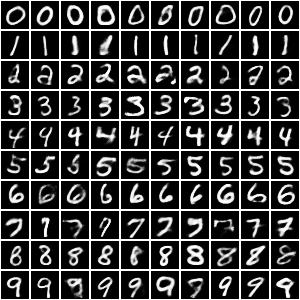
\includegraphics[scale=0.58]{epoch_3.jpg}
\caption{Generated Result}
\end{figure}
\par
The variational lower bound of the training and testing process is illustrated in Figure 7.
\begin{figure}[ht]
\centering
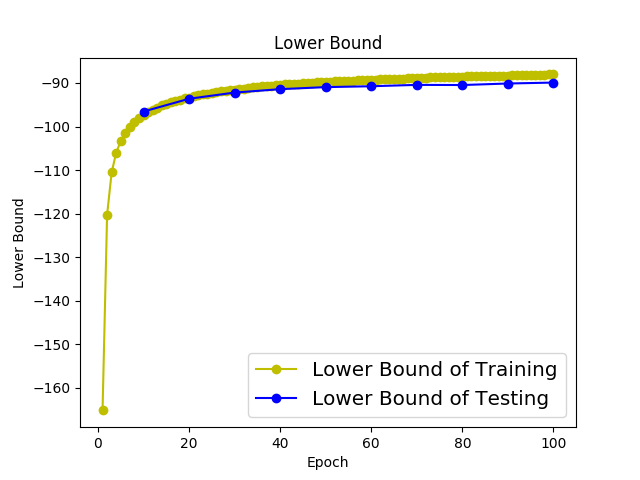
\includegraphics[scale=0.58]{Lower_Bound.png}
\caption{Lower Bound}
\end{figure}

\end{document}